\chapter{Lattice gass cellular automata}

History of Lattice Gass Cellular Automata began in 1973, when HPP model was proposed by Humphry, Pica and Picus.

Unfortunately, it could not do its job properly. For the reasons that we will explore in this chapter, its macroscopic limit did not converge to Navier-Stokes equations.

\bigskip

As we will see later, there came two different approaches how to make functioning LGCA and their common role model is this imperfect HPP.

Hence we will explain basic principles of LGCA on this model, and in subsequent chapters, we will "simply" upgrade it - either to FHP, Pair-interaction or their multi-dimensional variants.

\section{From CA to LGCA}

LGCA share many similarities with calular automata that we already saw,
but we need to be aware of the differences.

In general, LGCA is composed of regular clusters of cells - so called nodes. They are arranged in N-dimensional regular lattice.

Lattice of HPP is the simple rectangular 2D grid. At every point of a grid, there is node sitting in, and this node is composed of 4 cells, see Figure~\ref{rectangular}.

\begin{figure}[htbp]
 \centering
 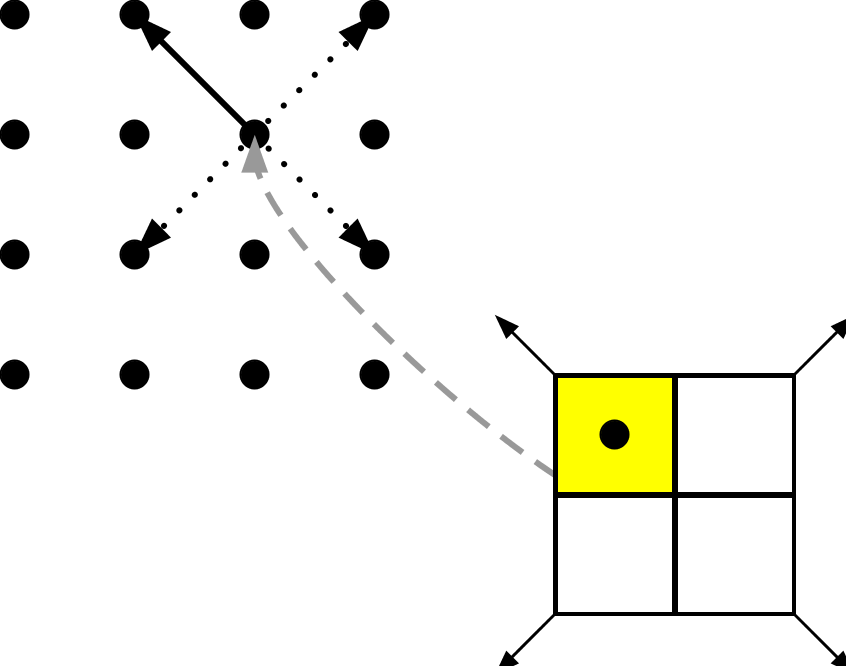
\includegraphics[width=0.6\textwidth]{./img/hpp}
 \label{rectangular}
 \caption{Rectangular grid}
\end{figure}

Each cell of the node can be in two states - empty (white square on the figure~\ref{rectangular}), or occupied by particle (yellow square on figure~\ref{rectangular}).
We see that particle in the upper-left square head to the upper-left node.


\section{Update rule}
For any LGCA model, update is done in two subsequent steps, collision and propagation.

In HPP, there are only two collision configuration, and one collision rule that guide them, see Figure~\ref{hpp-colision}.

\begin{figure}
 \centering
 \includegraphics[width=0.6\textwidth]{./img/hpp_col}
 \label{hpp-colision}
 \caption{HPP colisions}
\end{figure}

We see this configurations are symmetric. The first configuration is resolved to the other and vice versa.

It is easy to understand that there are no other collision configurations and collision rules. If any other state gets changed, it would break the conservation of momentum and would be physically unrealistic.

\section{Propagation:}

After the collision is resolved, propagation follows.
During propagation, particle from the upper-left cell moves to the upper-left node, and will occupy they same cell (with the same velocity vector), so that momentum is also conserved by the propagation.

\begin{figure} [h]
 \centering
 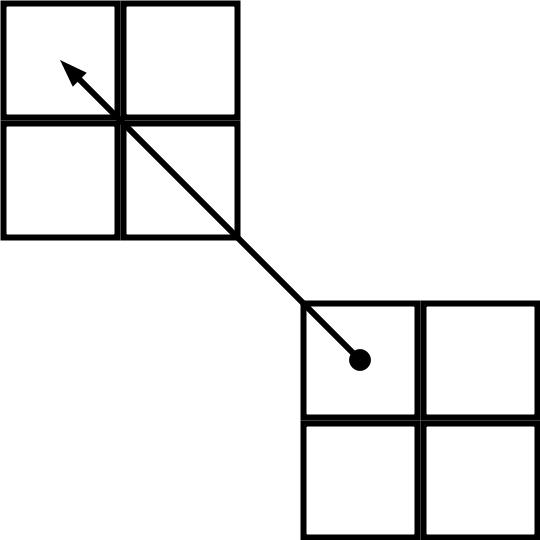
\includegraphics[width=0.3\textwidth]{./img/propleft}
 \label{hpp-colision}
 \caption{Propagation of particle from upper-left cell}
\end{figure}

\bigskip

\textbf{Conservation laws:}

We already made a note, that collision and propagation conserve momentum, and they obviously conserve mass, since particles are neither created, nor anihilated in these processes. 
Let us inspect these conservation laws in the more depth by considering symmetries of this model.

Suppose we are using periodic boundary condition. Then, the finite rectangular grid of HPP is actually a torus. It is easy to imagine that if we shift the grid by the discrete step (of length 1), we get the very same torus.
So this rectangular grid of HPP is symmetric with respect to translation.
As we know by Norther's theorems, translational symmetry implies conservation of momentum.

\bigskip

Also, the grid possesses some rough rotational symmetry - rotating the grid by 90 degrees, we get the same grid.

However, this rotation by 90 degrees is too crude, and so HPP do not preserve the angular momentum. This is the flaw of the model that cannot be overlooked - HPP do not preserve all physical quantities that Navier-Stokes equation would suggest.

Its another flaw goes in the opposite direction. HPP preserves quantities that are non-physical - so called spurious invariant.

Consider orientation of particles in Fig.\ref{hpp-colision} before colission.
One particle heads to north-east, the other south-west.
After the collision, one particle heads to north-west, other particle to south-east.
So the number of particles heading to the south, east, north and west do not change by collision (and neither by propagation). It is invariant as the time goes by.

To assert it more scientifistically, let us rozlozit the total momentum into the directions of lattice velocities
\begin{align} 
P = P_N + P_S + P_E + P_W.
\end{align}
This total momentum $P$ is correctly conserved by HPP, but also quantities
\begin{align} \label{zanet}
P_{spur1} = P_N + P_E - P_S - P_W
\end{align}
and
\begin{align}
P_{spur2} = P_N + P_W - P_S - P_E
\end{align}
are conserved, although these quantities have no physical counterparts.

\bigskip

To conclude this chapter and finish-off the HPP, it is physically implausible because
\begin{enumerate}
\item angular momentum is not conserved due to insufficient rotational symmetry,
\item other non-physical quantities, so called \textit{spurious invariants} are conserved.
\end{enumerate}

Although it is flawed model, it sparked interest of many bright minds and various successful LGCAs evolved from HPP. In the next chapter, we will introduce first successful branch of physically relevant LGCAs, the FHP model.